\documentclass[
	%parspace, % Add vertical space between paragraphs
	%noindent, % No indentation of first lines in each paragraph
	%nohyp, % No hyphenation of words
	%twoside, % Double sided format
	%draft, % Quicker draft compilation without rendering images
	%final, % Set final to hide todos
]{elteikthesis}[2023/04/10]

% The minted package is also supported for source highlighting
% See minted-intregration.tex for example
%\usepackage[newfloat]{minted}

% Document's metadata
\title{Title of the thesis} % title
\date{2023} % year of defense

% Author's metadata
\author{John Smith}
\degree{Computer Science BSc}

% Superivsor(s)' metadata
\supervisor{John Doe} % internal supervisor's name
\affiliation{Assistant Lecturer} % internal supervisor's affiliation
%\extsupervisor{Jane Doe} % external supervisor's name
%\extaffiliation{Senior Developer} % external supervisor's affiliation

% University's metadata
\university{Eötvös Loránd University} % university's name
\faculty{Faculty of Informatics} % faculty's name
\department{Dept. of Software Technology and Methodology} % department's name
\city{Budapest} % city
\logo{elte_cimer_szines} % logo

% Add bibliography file
\addbibresource{elteikthesis.bib}

% The document
\begin{document}

% Set document language
%\documentlang{hungarian}
\documentlang{english}

% List of todos (not in the final document)
%\listoftodos[\todolabel]

% Title page (mandatory)
\maketitle
% Topic declaration page (mandatory) - can also be attached instead
%\includepdf{topicdeclaration.pdf}

% Table of contents (mandatory)
\tableofcontents
\cleardoublepage

% Main content
\chapter{Introduction}
\label{ch:intro}

Lorem ipsum dolor sit amet, consectetur adipiscing elit. In eu egestas mauris. Quisque nisl elit, varius in erat eu, dictum commodo lorem. Sed commodo libero et sem laoreet consectetur. Fusce ligula arcu, vestibulum et sodales vel, venenatis at velit \cite{dahl1972structured}. Aliquam erat volutpat. Proin condimentum accumsan velit id hendrerit. Cras egestas arcu quis felis placerat, ut sodales velit malesuada. Maecenas et turpis eu turpis placerat euismod.\footnote{Maecenas a urna viverra, scelerisque nibh ut, malesuada ex.}

Aliquam suscipit dignissim tempor. Praesent tortor libero, feugiat et tellus porttitor, malesuada eleifend felis. Orci varius natoque penatibus et magnis dis parturient montes, nascetur ridiculus mus \cite{cormen2009algorithms,krasner1988mvc}. Nullam eleifend imperdiet lorem, sit amet imperdiet metus pellentesque vitae. Donec nec ligula urna. Aliquam bibendum tempor diam, sed lacinia eros dapibus id. Donec sed vehicula turpis. Aliquam hendrerit sed nulla vitae convallis. Etiam libero quam, pharetra ac est nec, sodales placerat augue. \citeauthor{dijkstra1979goto} praesent eu consequat purus \cite{dijkstra1979goto}. 

\cleardoublepage

\chapter{User documentation}
\label{ch:user}
The ability to improve the scalability, agility, and dependability of applications in cloud environments has led to a rise in the popularity of cloud-native development in recent years. The foundation of this strategy is containerization, which offers a standardized and portable way to package and distribute software.

The industry standard for scaling up containerized application management is Kubernetes, a well-known container orchestration technology. In addition to tools for automating these procedures, it offers a complete set of primitives for deploying, scaling, and managing containerized applications.

For automated web browser testing of online applications, particularly in continuous integration and continuous delivery (CI/CD) pipelines, Selenium, an open-source testing framework, is crucial. In a cloud-native setting, Selenium testing integration with Kubernetes is essential.

This project implements a Go-based Kubernetes operator, a custom controller that extends the Kubernetes API and automates the deployment and management of Selenium tests in a Kubernetes cluster while making it easy to integrate into industry-standard monitoring and alerting chains.

This documentation will cover all operator usage aspects, including installation, configuration, and customization. We will also provide examples of how to use the operator to automate the execution of Selenium tests and how to integrate it with other Kubernetes-native tools and services.

\section{Prerequisites of employing the operator}

The operator is designed to be utilized in Kubernetes clusters of business scale, whether they are hosted on public cloud servers or on-premise servers. Although the operator was designed with performance in mind, neither Kubernetes, Selenium hubs nor Prometheus monitoring stacks are intended for local development; however, they are all necessary to show the project's feasibility. Since this tutorial will show it on a local Kubernetes cluster, be aware that hardware-related issues could occur.

Requirements are the followings:
\begin{itemize}
	\item Kubernetes cluster (minikube in the manual)
	\item Shell environment (Linux/Mac OS or Windows with WSL)
	\item kubectl CLI tool
	\item make CLI tool
	\item selenium test exported to .side format
	\item rented or self-managed Selenium Hub service (moon in the manual) 
	\item operator-managed Prometheus in the Kubernetes cluster (kube-prometheus in the manual)
	\item Helm CLI tool for deploying all the above
\end{itemize}

This manual will demonstrate setting up the following Kubernetes environment before deploying the first automated test:

\begin{figure}[H]
	\centering
	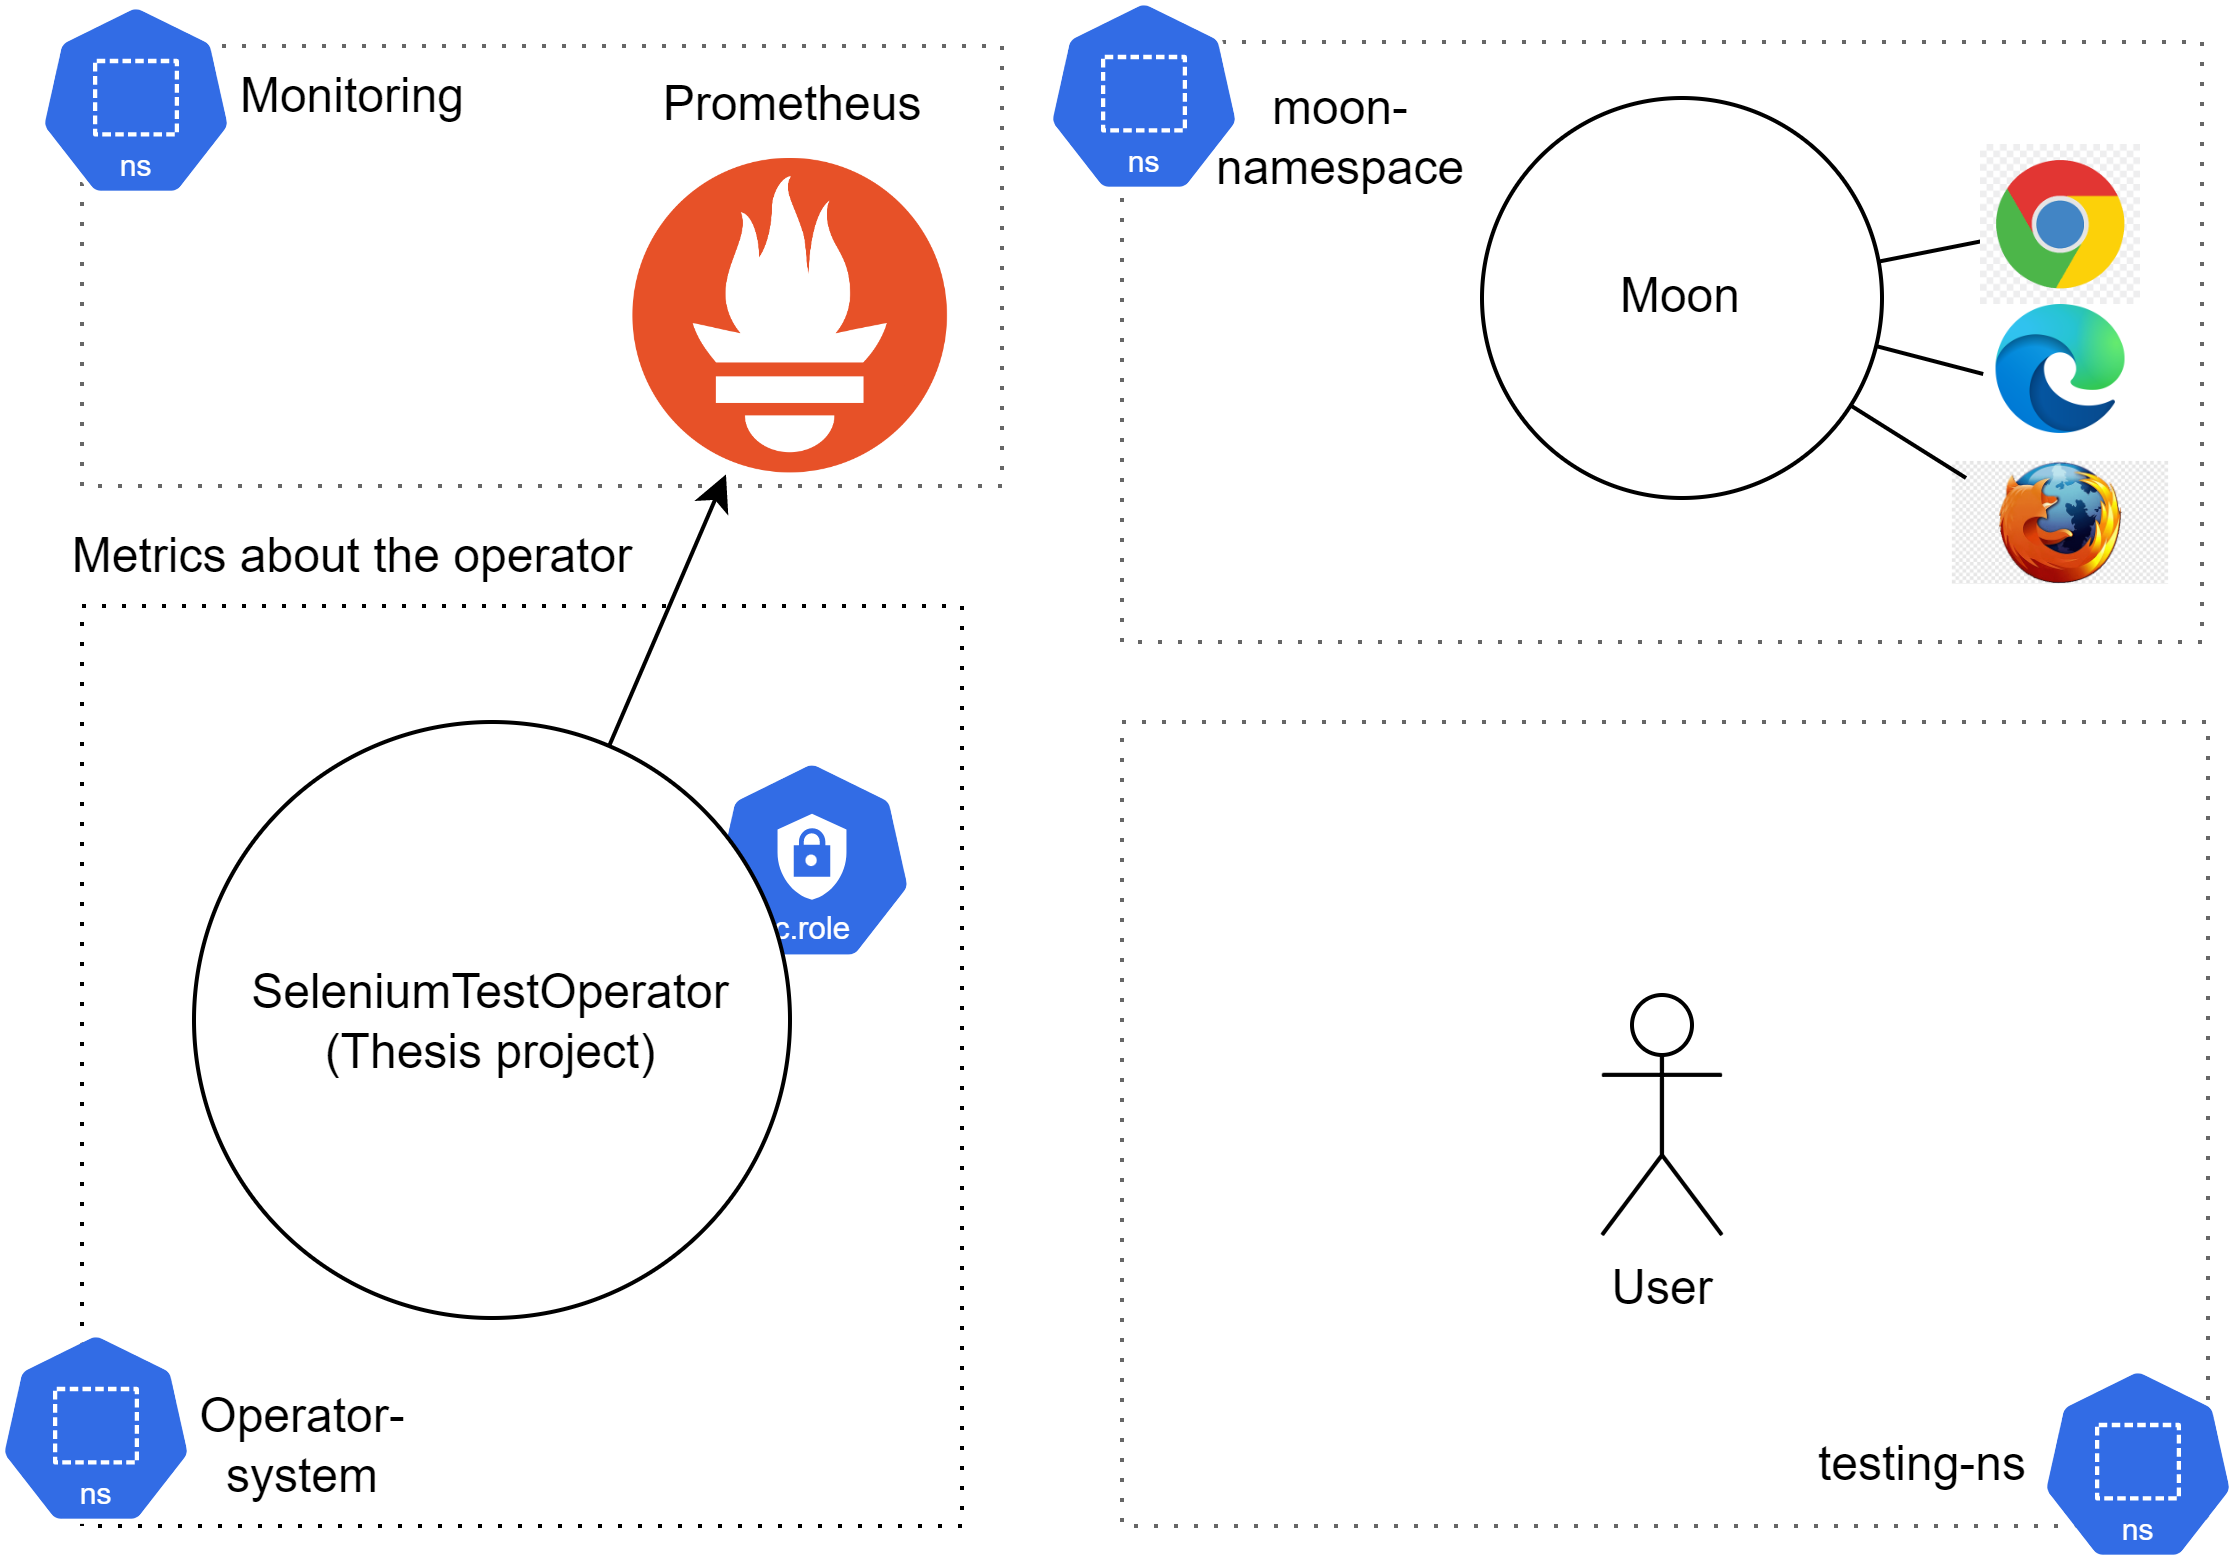
\includegraphics[width=1\textwidth]{before_tests}
	\label{fig:before_tests}
	\caption{Architecture without running tests}
\end{figure}

\subsection{Installing a Minikube cluster}

Before setting up the tools required for running Selenium tests with Kubernetes, a few prerequisites need to be installed. These prerequisites include a Kubernetes cluster, a virtualization tool for Minikube, a shell environment, the kubectl CLI tool, the make CLI tool, and a Selenium test exported to .side format. In this guide, we'll go through each of these prerequisites in detail and show you how to install them on your machine. Once these prerequisites are in place, we can move on to setting up the SeleniumTest Operator and creating custom resources for running Selenium tests.

Before everything else, Windows users has to install WSL by opening the Microsoft Store on Windows and search for "Ubuntu" or any other Linux distribution of choice and launch it.

From now on, shell environment will be used universally between operating systems, meaning shell on either Linux, Mac OS or Windows' WSL.

\begin{itemize}
	\item First of all, intall kubectl:

	\begin{itemize}
		\item In the shell terminal, run the following commands:	
		\lstset{caption={Installing kubectl}}
		\begin{lstlisting}[language=bash]
			curl -LO "https://storage.googleapis.com/kubernetes-release/release/$(curl -s https://storage.googleapis.com/kubernetes-release/release/stable.txt)/bin/linux/amd64/kubectl"
			chmod +x ./kubectl
			sudo mv ./kubectl /usr/local/bin/kubectl
		\end{lstlisting}

		\item Verify that kubectl is installed:
		\lstset{caption={Verifying kubectl}}
		\begin{lstlisting}[language=bash]
			kubectl version --short
		\end{lstlisting}
	\end{itemize}

	\item Secondly, to install make, run the following command in the shell terminal:
	\lstset{caption={Installing make}}
	\begin{lstlisting}[language=bash]
		sudo apt-get install build-essential
	\end{lstlisting}
	
	\item Thirdly, to install helm, run In the shell terminal:
	\lstset{caption={Installing helm}}
	\begin{lstlisting}[language=bash]
		curl -fsSL -o get_helm.sh https://raw.githubusercontent.com/helm/helm/main/scripts/get-helm-3
		chmod 700 get_helm.sh
		./get_helm.sh
	\end{lstlisting}

	\item Fourthly, to install and configure Minikube:

	\begin{itemize}
		\item Windows users:	
		\begin{itemize}
			\item Open your web browser and go to the Minikube releases page on GitHub (https://github.com/kubernetes/minikube/releases).
			\item Find the latest release for Windows and download the executable file (e.g., minikube-windows-amd64.exe).
			\item Move the downloaded executable to a folder that is included in your PATH environment variable. For example, you can move it to the "C:\\Windows\\System32" folder.
			\item Install Docker desktop for Minikube from its offical site: https://www.docker.com/products/docker-desktop/
		\end{itemize}
		\item Linux users:
		\lstset{caption={Installing minikube cli for Linux}}
		\begin{lstlisting}[language=bash]
			curl -LO https://storage.googleapis.com/minikube/releases/latest/minikube-linux-amd64
			sudo install minikube-linux-amd64 /usr/local/bin/minikube
		\end{lstlisting}
		\item Mac users:
		\begin{itemize}
			\item Install Homebrew by running the following command in Terminal:
			\lstset{caption={Installing homebrew cli for Mac}}
			\begin{lstlisting}[language=bash]
				/bin/bash -c "$(curl -fsSL https://raw.githubusercontent.com/Homebrew/install/HEAD/install.sh)"
			\end{lstlisting}

			\item Once Homebrew is installed, you can install minikube by running the following command in Terminal:
			\lstset{caption={Installing minikube cli for Mac}}
			\begin{lstlisting}[language=bash]
				brew install minikube
			\end{lstlisting}
		\end{itemize}
		\item After the installation is complete, validate it with the following command:
		\lstset{caption={Verifying minikube cli tool}}
		\begin{lstlisting}[language=bash]
			minikube version
		\end{lstlisting}	
	\end{itemize}

	\item Lastly, we need to start Minikube:
	\begin{itemize}
		\item Minikube startup under Windows:
		\lstset{caption={Starting minikube for Windows}}
		\begin{lstlisting}[language=bash]
			minikube start --cpus=4 --memory=8G --disk-size=30G --driver=docker
		\end{lstlisting}
		\item Minikube startup under MacOS:
		\lstset{caption={Starting minikube for MacOS}}
		\begin{lstlisting}[language=bash]
			minikube start --cpus=4 --memory=8G --disk-size=20G --driver=hyperkit
		\end{lstlisting}
		\item Minikube startup under Linux
		\lstset{caption={Starting minikube for Linux}}
		\begin{lstlisting}[language=bash]
			minikube start --cpus=4 --memory=8G --disk-size=20G --driver kvm2
		\end{lstlisting}
	\end{itemize}
	\item Even though Moon advises against using Docker as a driver, it is necessary from a networking perspective for Windows users in order to be able to access the cluster from WSL. Providing Minikube with more resources is strongly recommended if possible, but these should be the absolute minimum.
	\item Verify that Minikube is running:
	\lstset{caption={Verifying minikube cluster}}
	\begin{lstlisting}[language=bash]
		kubectl cluster-info
	\end{lstlisting}
\end{itemize}

\subsection{Solving kubectl connection problem on Windows}

A configuration file for the kubectl command-line tool for Kubernetes can be found at "~/.kube/config". In addition to the credentials required for cluster authentication, it indicates the Kubernetes cluster with which kubectl should communicate.

Depending on the setup, when installing Minikube, it creates a Kubernetes cluster in a virtual machine or a container. Minikube changes the computer's "~/.kube/config" file to set up kubectl to use this new cluster automatically. As a result, kubectl can communicate with the Minikube cluster.

Windows users encounter a problem since Minikube sets the configuration file at the Windows operating system level, whereas kubectl refers to the configuration file contained in the WSL distribution.

\begin{figure}[H]
	\centering
	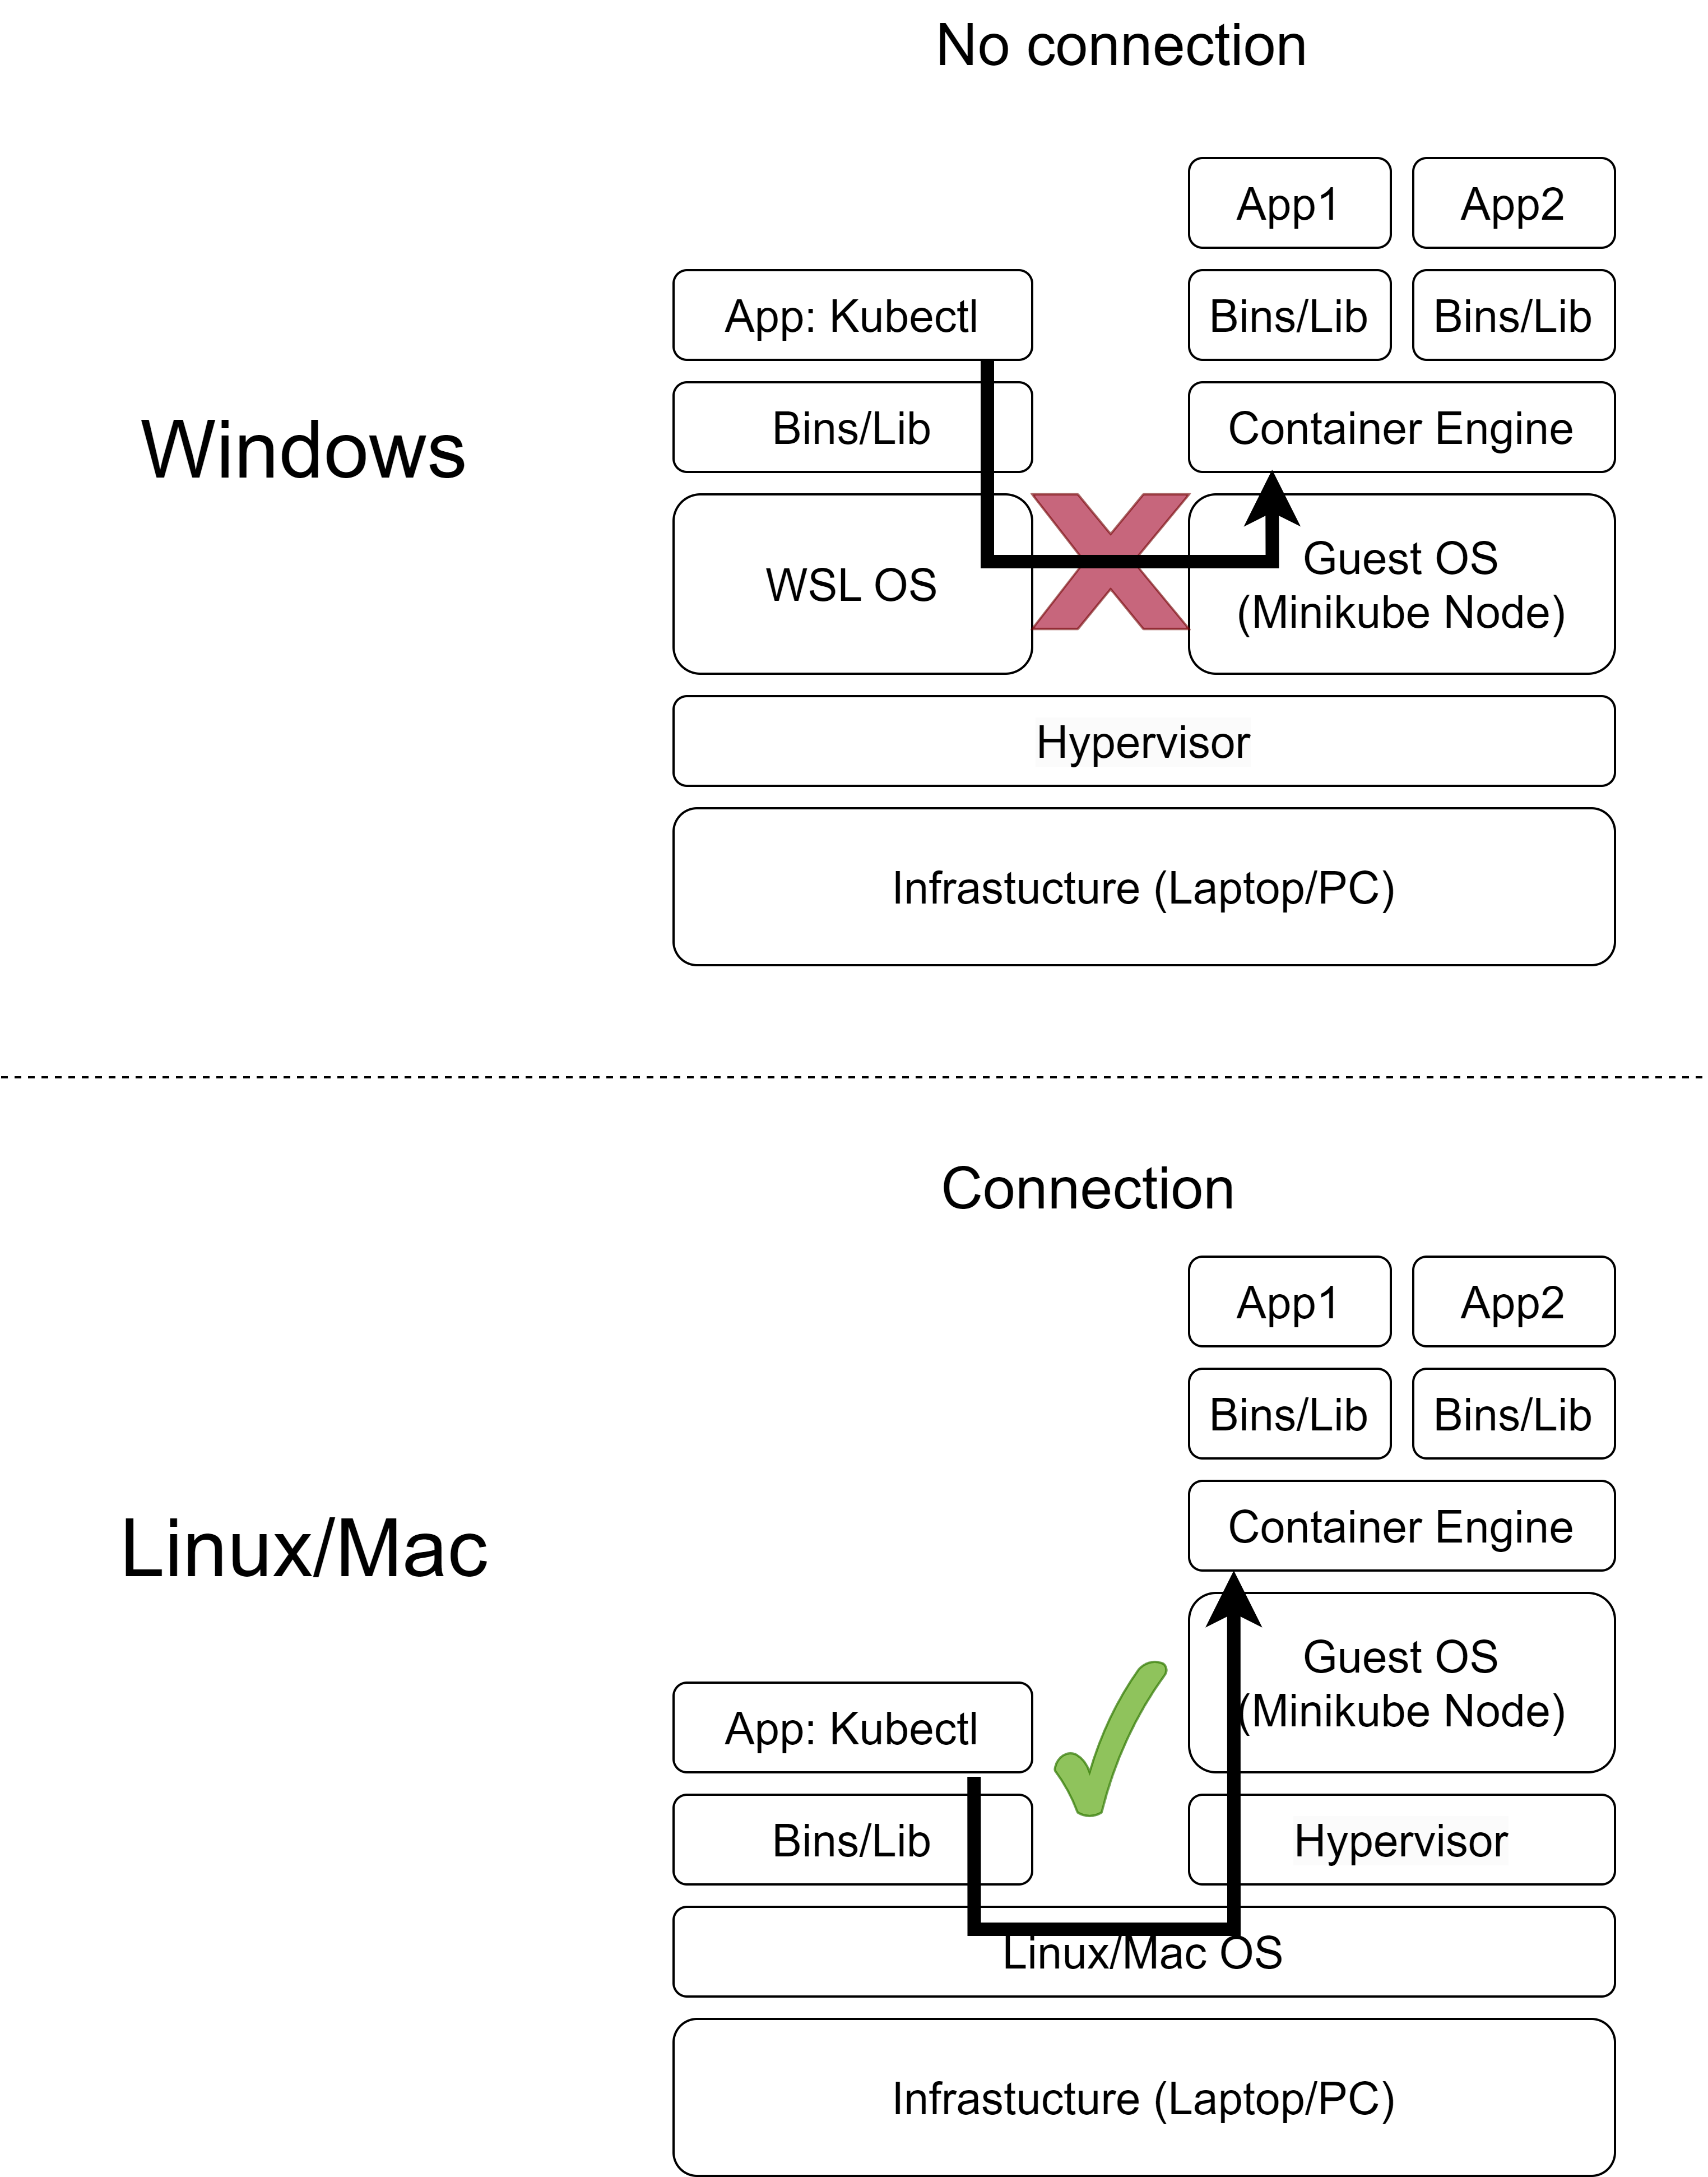
\includegraphics[width=1\textwidth]{window_virtualisation}
	\label{fig:window_virtualisation}
	\caption{Virtualization difference between WSL and Unix systems}
\end{figure}

We must manually generate the kubeconfig file based on the one Minikube created to fix the problem. Although the two files will be very similar, there will be a few minor adjustments because one was created for Windows and the other for Linux.

This is how the new kubeconfig file should appear:
\lstset{caption={Example kubeconfig file}}
\begin{lstlisting}[language=bash]
	apiVersion: v1
	clusters:
	- cluster:
		certificate-authority: /mnt/c/Users/Your_User/.minikube/ca.crt
		extensions:
		- extension:
			last-update: Sat, 18 Mar 2023 17:26:55 CET
			provider: minikube.sigs.k8s.io
			version: v1.27.0
		  name: cluster_info
		server: https://127.0.0.1:8443
	  name: minikube
	contexts:
	- context:
		cluster: minikube
		extensions:
		- extension:
			last-update: Tue, 02 May 2023 22:28:36 CEST
			provider: minikube.sigs.k8s.io
			version: v1.27.0
		  name: context_info
		namespace: default
		user: minikube
	  name: minikube
	current-context: minikube
	kind: Config
	preferences: {}
	users:
	- name: minikube
	  user:
		client-certificate: /mnt/c/Users/Your_User/.minikube/profiles/minikube/client.crt
		client-key: /mnt/c/Users/Your_User/.minikube/profiles/minikube/client.key
\end{lstlisting}

After creating the file, run the following command in the WSL terminal:
\lstset{caption={Setting Kubeconfig}}
\begin{lstlisting}[language=bash]
	export KUBECONFIG=path/to/your/kubeconfig
\end{lstlisting}

Lastly, verify that Minikube is reachable:
\lstset{caption={Validate Minikube}}
\begin{lstlisting}[language=bash]
	kubectl cluster-info
\end{lstlisting}

\subsection{Deploying the required applications to the cluster}

This section will set up the kube-prometheus, Moon, and seleniumTest operator on our Kubernetes cluster. These tools are essential for testing and monitoring our cluster to ensure it runs smoothly and dependably. For our cluster, kube-prometheus offers a reliable monitoring solution that enables us to keep an eye on critical parameters like resource utilization and application performance. While the SeleniumTest Operator automates the deployment and upkeep of those tests in our Kubernetes cluster, Moon is a Selenium Grid implementation that we will use to run our Selenium tests. 

We will only deploy the Prometheus operator portion of the kube-prometheus stack because of the limited hardware resources available locally, as the other components are useless for this demonstration. Enter the operator repository to get started, then execute the following commands:
\lstset{caption={Deploying Prometheus operator}}
\begin{lstlisting}[language=bash]
	kubectl apply --server-side -f prometheus/setup
	kubectl wait --for condition=Established --all CustomResourceDefinition --namespace=monitoring
	kubectl apply -f prometheus/
\end{lstlisting}

Whenever there are issues, visit kube-prometheus's official github page for more details on how to deploy it: https://github.com/prometheus-operator/kube-prometheus

The following commands will deploy Moon, the Selenium Grid implementation, so that the tests may be run:
\lstset{caption={Installing moon}}
\begin{lstlisting}[language=bash]
	helm repo add aerokube https://charts.aerokube.com/
	helm repo update
	kubectl create namespace moon
	helm upgrade --install -f moon_values.yaml -n moon moon aerokube/moon2
\end{lstlisting}
Ingress controller is disabled in the moon_values.yaml file because we won't attempt to contact Moon from outside the cluster.

The seleniumTest operator can then be deployed; perform the following steps from the operator's repository:
\lstset{caption={Deploying of operator}}
\begin{lstlisting}[language=bash]
	make deploy IMG=quay.io/molnar_liviusz/selenium-test-operator:v0.0.24
\end{lstlisting}

Finally, we need to create and change the context to the namespace for our project, where we will launch all of the Selenium tests:
\lstset{caption={Creating testing namespace}}
\begin{lstlisting}[language=bash]
	kubectl create namespace testing-ns
	kubectl config set-context --current --namespace=testing-ns
\end{lstlisting}

Downloading Lens is advised for simpler cluster management (https://k8slens.dev/). Lens offers a straightforward and understandable graphical user interface for controlling Kubernetes clusters. Users can navigate and change resources, view their cluster's current state, and keep an eye on performance indicators in real time. Additionally, Lens supports numerous clusters and offers a single location for managing them all. Lens is a fantastic alternative for developers and system administrators who need to work with Kubernetes on a regular basis due to its user-friendly interface and extensive feature set.

The outcome of all this is that we now have our cluster configured, achieving the cluster state shown in the previous architecture diagram, with the seleniumTest operator, Prometheus, to query our operator's metrics (including the test results), and Moon deployment as a Selenium Grid implementation. The test recordings are the final component needed to deploy tests.

\subsection{Recorded selenium tests with Selenium IDE}

Selenium IDE is a browser extension that may be used to record user interactions with a web application. The user can export the recorded interactions in the ".side" (Selenium Integrated Development Environment) file format once the recording is finished. This file may then be used with Selenium WebDriver to reliably and repeatedly automate the same interactions. The ".side" file provides details on the actions taken, the web page elements that were the targets, and any additional data like input values or anticipated outcomes. Developers and testers can save time and effort while creating and maintaining automated tests by utilizing Selenium IDE to record and export interactions into a ".side" file.

To create a selenium test, open the extension > Record a new test in a new project > add a project name > add the URL where the browser should open at the beginning of the test > start recording > finish recording:

\begin{figure}[H]
	\centering
	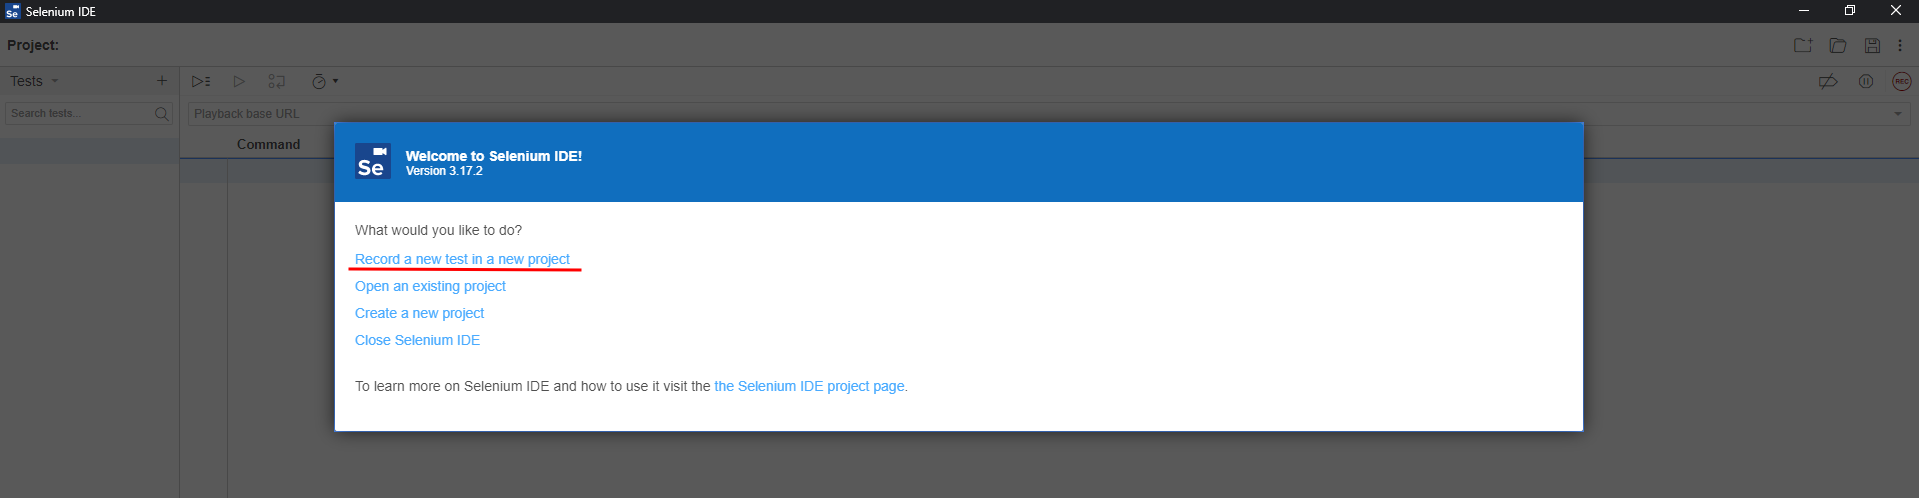
\includegraphics[width=1\textwidth]{seleniumide1}
	\label{fig:seleniumide1}
	\caption{SeleniumIDE 1}
\end{figure}

\begin{figure}[H]
	\centering
	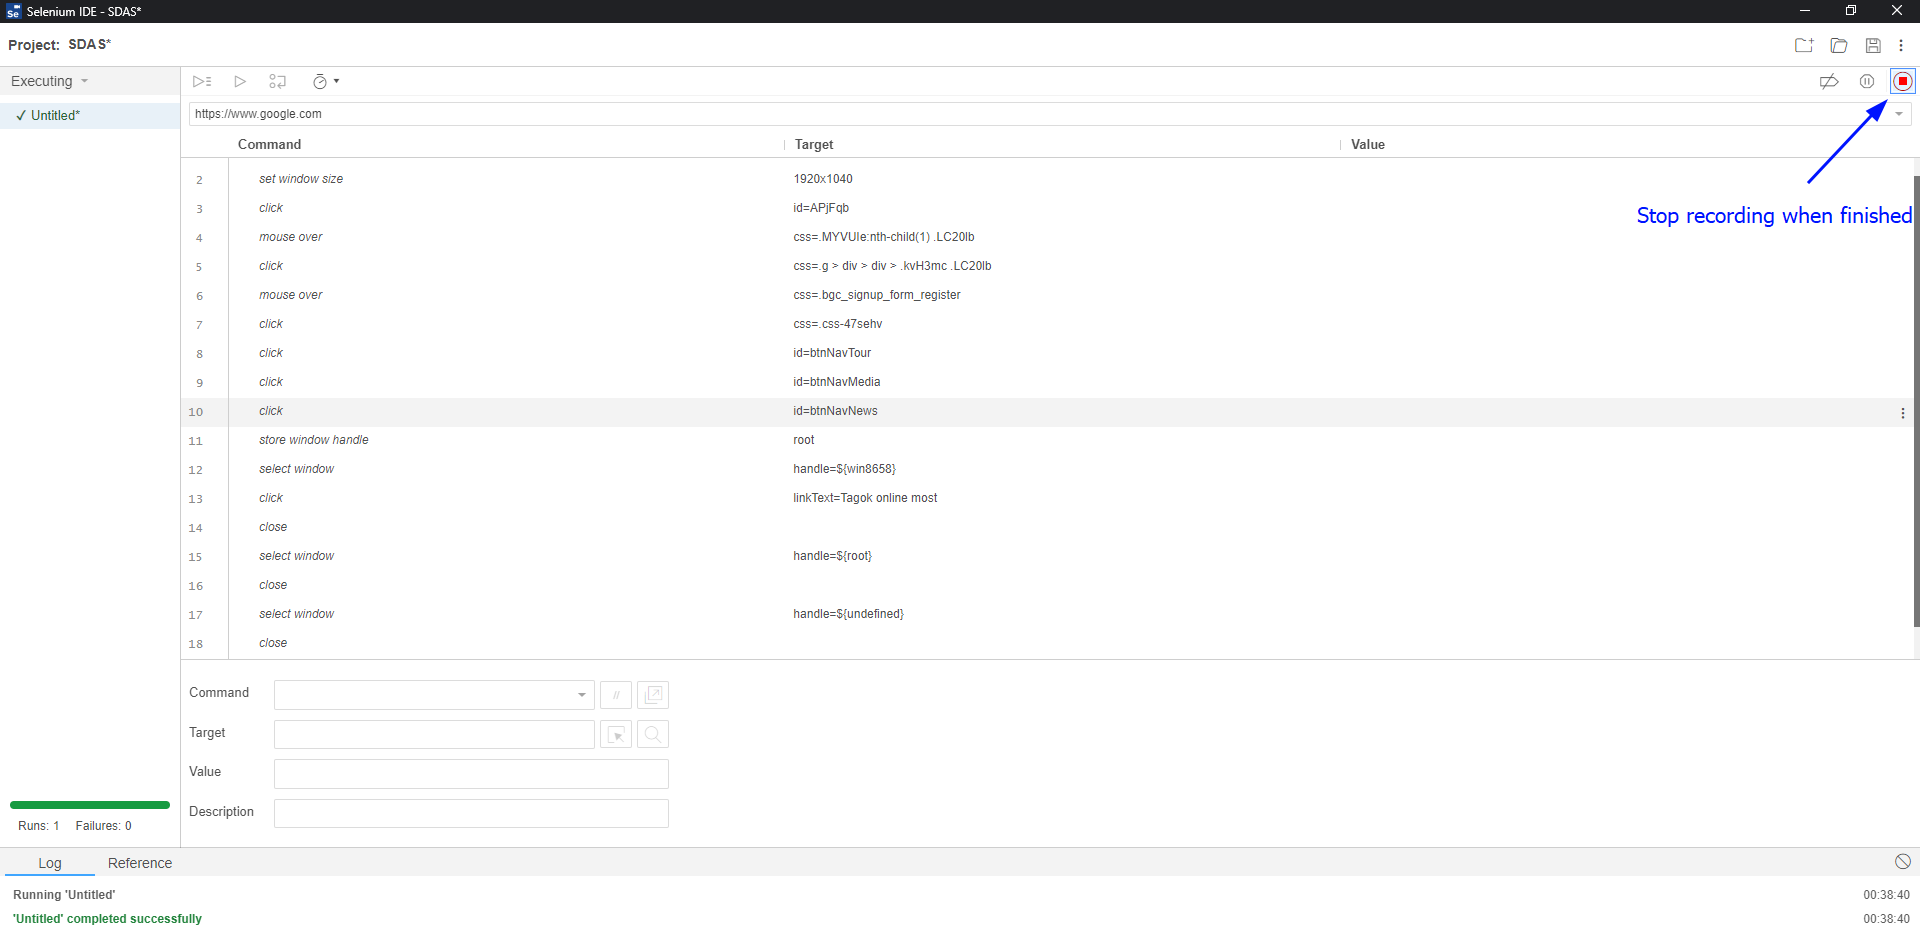
\includegraphics[width=1\textwidth]{seleniumide2}
	\label{fig:seleniumide2}
	\caption{SeleniumIDE 2}
\end{figure}

Replacing the actions' default target variables with a specific XPath target is advised to increase test reliability. Recommend doing this while utilizing the "XPath Helper" browser plugin and the browsers' inspect mode:

\begin{figure}[H]
	\centering
	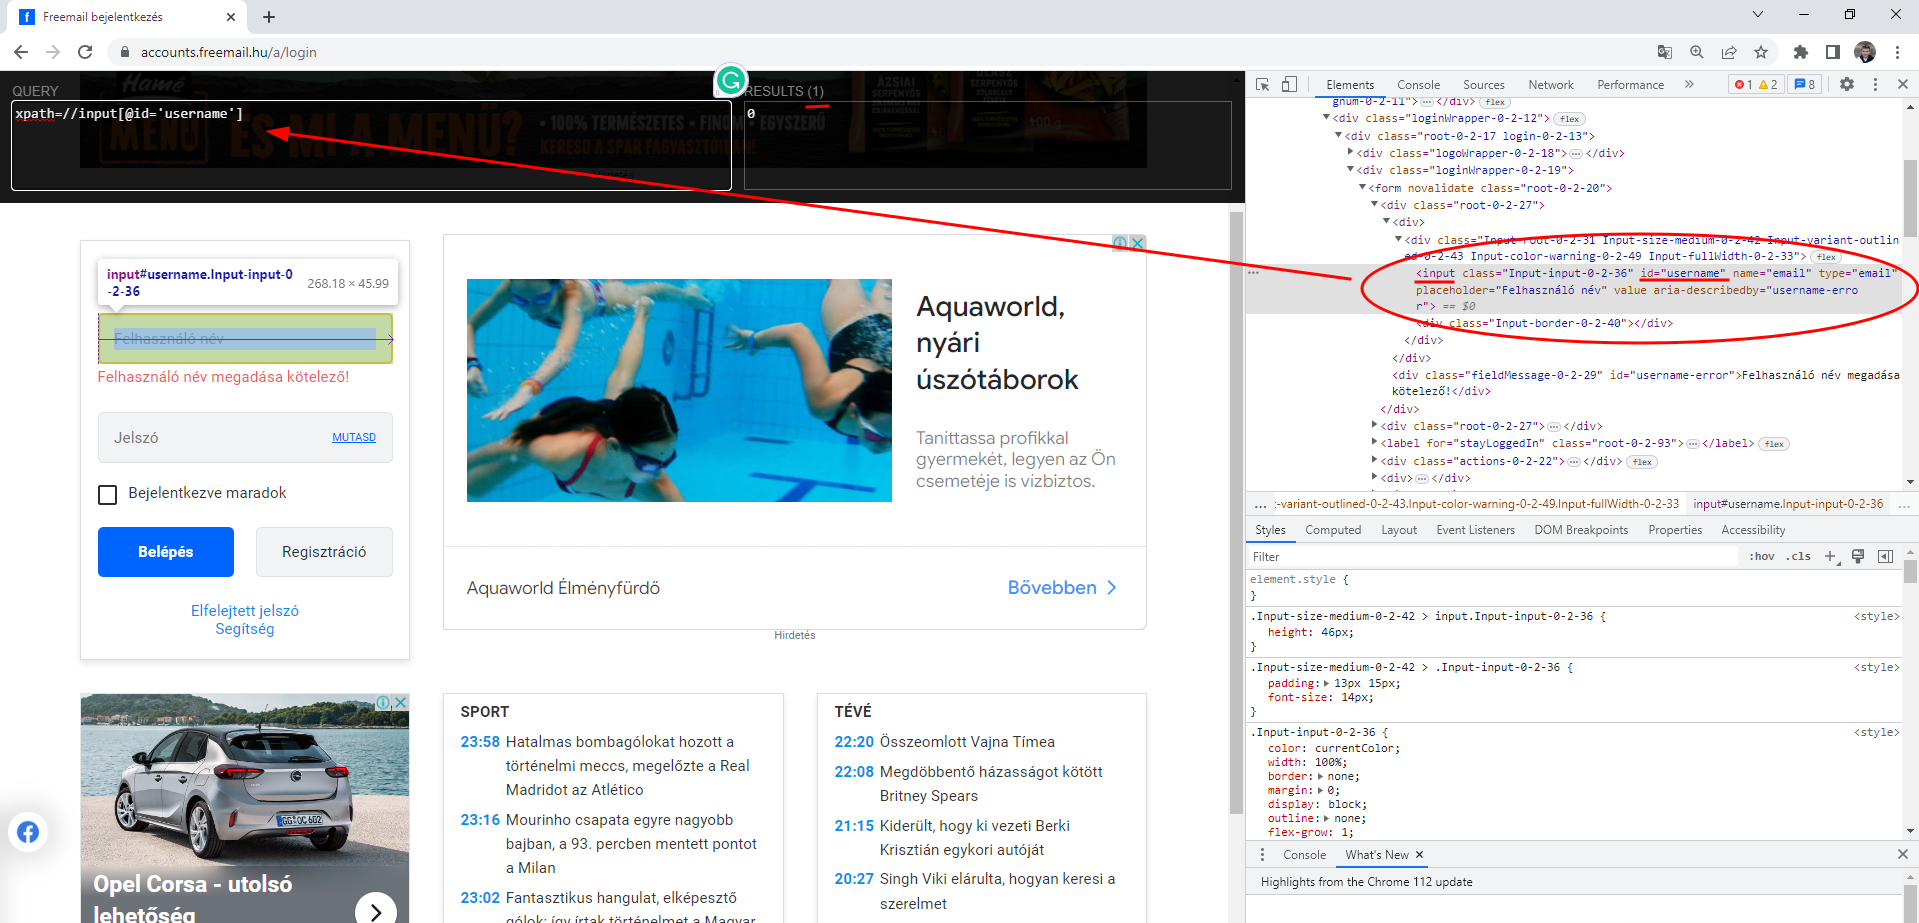
\includegraphics[width=1\textwidth]{xpathhelper}
	\label{fig:xpathhelper}
	\caption{XPath Helper}
\end{figure}

\begin{figure}[H]
	\centering
	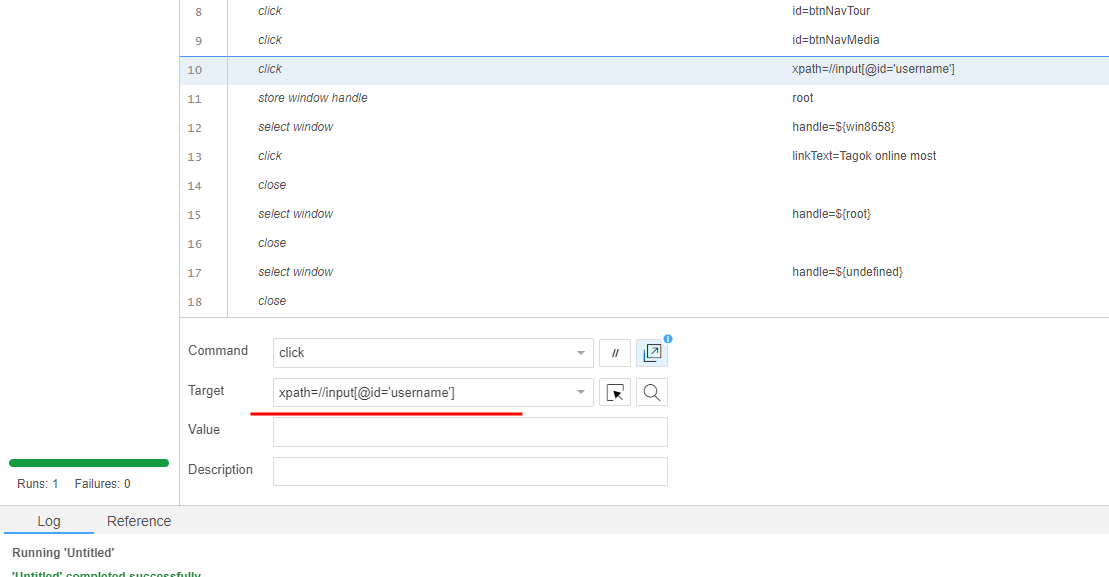
\includegraphics[width=1\textwidth]{seleniumide3}
	\label{fig:seleniumide3}
	\caption{SeleniumIDE 3}
\end{figure}

Several tests can be conducted within a single test project, and sophisticated Selenium Grid implementations, such as Moon, can perform these tests in a paralyzed fashion to increase efficiency and shorten the testing time. Once finished, save the project into the default .side extension.

\section{Deploying Automated Selenium Tests}

Automating the running of Selenium tests on a Kubernetes cluster requires a configuration file for the test, a ConfigMap that stores the .side file. A custom resource called SeleniumTest needs to be created to define the desired state of the test, such as the image to be used, the Selenium Grid to connect to, and the schedule for running the test. With these two components in place, Kubernetes can automatically run the Selenium test according to the specified schedule, greatly simplifying web application testing.

The configmap looks resembles the following:
\lstset{caption={Example configmap with .side test}}
\begin{lstlisting}[language={Go}]
	apiVersion: v1
	kind: ConfigMap
	metadata:
	  name: testcode
	  namespace: testing-ns
	data:
	  # file-like keys
	  exampletest.side: |
		{
		  "id": "02faada0-52b8-49fe-95cc-d403a5ef9dcd",
		  "version": "2.0",
		  "name": "Operator",
		  "url": "https://accounts.freemail.hu",
		  "tests": [{
			"id": "cf677198-9658-455c-b524-c2fa55ad59f7",
			"name": "login",
			"commands": [{
			  "id": "31de9648-b82a-4322-90da-65ee6a89a9f5",
			  .
			  .
			  .
\end{lstlisting}

The following is the syntax for the seleniumTest custom resource:
\lstset{caption={SeleniumTest CR yaml format}}
\begin{lstlisting}[language={Go}]
	apiVersion: selenium.mliviusz.com/v1
	kind: SeleniumTest
	metadata:
		labels:
			app.kubernetes.io/name: seleniumtest
			app.kubernetes.io/instance: seleniumtest-sample
			app.kubernetes.io/part-of: operator
			app.kubernetes.io/managed-by: kustomize
			app.kubernetes.io/created-by: operator
		name: seleniumtest-sample
		namespace: testing-ns
	spec:
		schedule: "*/2 * * * *"
		repository: quay.io
		image: molnar_liviusz/selenium-test-runner
		tag: v0.0.10
		configMapName: testcode
		retries: "3"
		seleniumGrid: "http://moon.moon.svc:4444/wd/hub"
\end{lstlisting}

The SeleniumTest object's desired state is specified in the spec section of the custom resource with the following variables:

\begin{itemize}
	\item repository: specifies the repository for the Docker image.
	\item image: The Docker image that will be used to execute the test is specified by this option. This image is also part of the thesis project
	\item tag: This parameter specifies the tag for the Docker image.
	\item retries: The number of times the test should be rerun if it fails is specified by this option. The test counts as a pass even if one is successful.
	\item schedule: This parameter specifies the schedule for the CronJob that runs the test.
	\item seleniumGrid: This parameter specifies the URL of the Selenium Grid for running the test.
\end{itemize}

To deploy the test, use the following commands:
\lstset{caption={Deploying example tests}}
\begin{lstlisting}[language=bash]
	kubectl apply -f testfiles/testcode-configmap.yaml
	kubectl apply -f testfiles/sample-seleniumtest.yaml
\end{lstlisting}

Following the previous steps, the test results can be viewed on Prometheus, where 0 means succes, 1 means the test failed:
\begin{figure}[H]
	\centering
	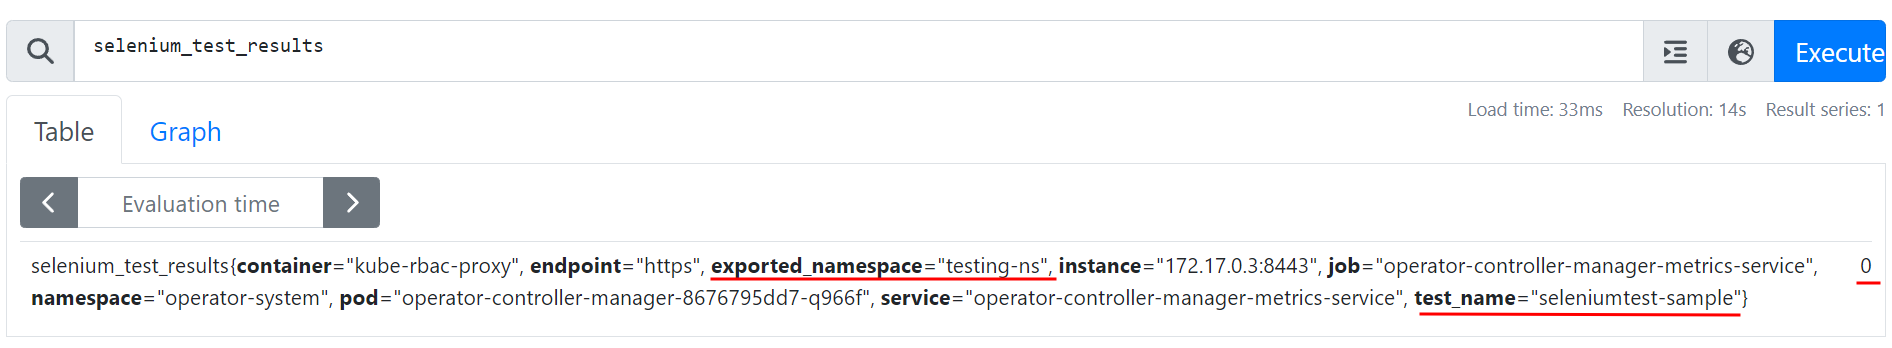
\includegraphics[width=1\textwidth]{prometheus_ui}
	\label{fig:prometheus_ui}
	\caption{Seleniumtest metric within Prometheus}
\end{figure}
\cleardoublepage

\chapter{Developer documentation}
\label{ch:impl}

This essay automates Selenium tests in a cloud-native environment using a Go-based Kubernetes operator. This section contains full usage instructions for this Kubernetes operator and in-depth explanations of its features, design philosophy, and supporting technologies.

The Kubernetes operator is a tool that automates the deployment, maintenance, and scaling of Selenium tests in a Kubernetes cluster, which will be covered in this documentation. It makes it simple for DevOps teams and developers to integrate Selenium testing into production workflows, guaranteeing that their cloud-native applications are extensively tested and optimized for performance, scalability, and dependability.

This documentation will provide all the information to know to take advantage of the capabilities of this Go-based Kubernetes operator for Selenium testing, whether you are an experienced Kubernetes developer or are just getting started with cloud-native application development. Therefore, let us get in and get to exploring!

\section{Understanding the underlying technologies}

Understanding the underlying technologies that enable the Go-based Kubernetes operator for Selenium testing is crucial before we go into its specifics. The necessity of introducing these technologies and their importance in the context of developing cloud-native applications will be covered in this section.

Due to its capacity to increase the scalability, agility, and dependability of applications running in a cloud environment, cloud-native application development has grown in popularity in recent years. The use of containerization, which offers a standardized and portable mechanism to bundle and distribute programs, is at the core of this strategy.

Popular container orchestration platform Kubernetes has become the de facto standard for scalably managing containerized applications. In addition to tools for automating these procedures, it offers a complete set of primitives for deploying, scaling, and managing containerized applications.

On the other hand, the open-source testing framework Selenium enables programmers to automate web browser testing for web applications. In the context of continuous integration and continuous delivery (CI/CD) pipelines, in particular, it has evolved into a crucial tool for maintaining the quality and performance of online applications.

It is vital to integrate Selenium testing with Kubernetes to use its advantages in a cloud-native environment. The Go-based Kubernetes operator is helpful in this situation. To automate the deployment and maintenance of Selenium tests in a Kubernetes cluster, a custom controller that extends the Kubernetes API is used.

Understanding the underlying technologies is crucial for successfully operating the Go-based Kubernetes operator for Selenium testing. By doing this, DevOps teams and developers may better understand the utility of this operator and utilize it to improve their processes for creating cloud-native applications.

\subsection{Differences between Virtual Machines and Containers}

Virtual machines and containers are two standard technologies in cloud computing and application deployment. Virtual machines and containers offer isolation and virtualization, but they differ in several important ways. The distinctions between virtual machines and containers are covered in this section.

Software-based simulations of physical devices are known as virtual machines. They execute a whole operating system on top of a hypervisor, emulating the entire hardware stack, including the processor, memory, and storage. Each virtual machine has its own virtualized hardware, operating system, and isolated environment in which it operates. As a result, it is possible to run many operating systems on a single physical machine and achieve total isolation.

On the other hand, containers are a minimal type of virtualization that works at the operating system level. Multiple applications can run on the same operating system instance thanks to containers, which use the host operating system kernel and share resources with other containers. Virtual machines can be replaced by more lightweight and practical containers, which speed up the deployment and scaling of applications.

One of the key distinctions is how virtual machines and containers use their resources. Resource wastage can occur because virtual machines need many resources to replicate a whole hardware stack. Contrarily, containers use resources better because they share the host operating system kernel.

\begin{figure}[H]
	\centering
	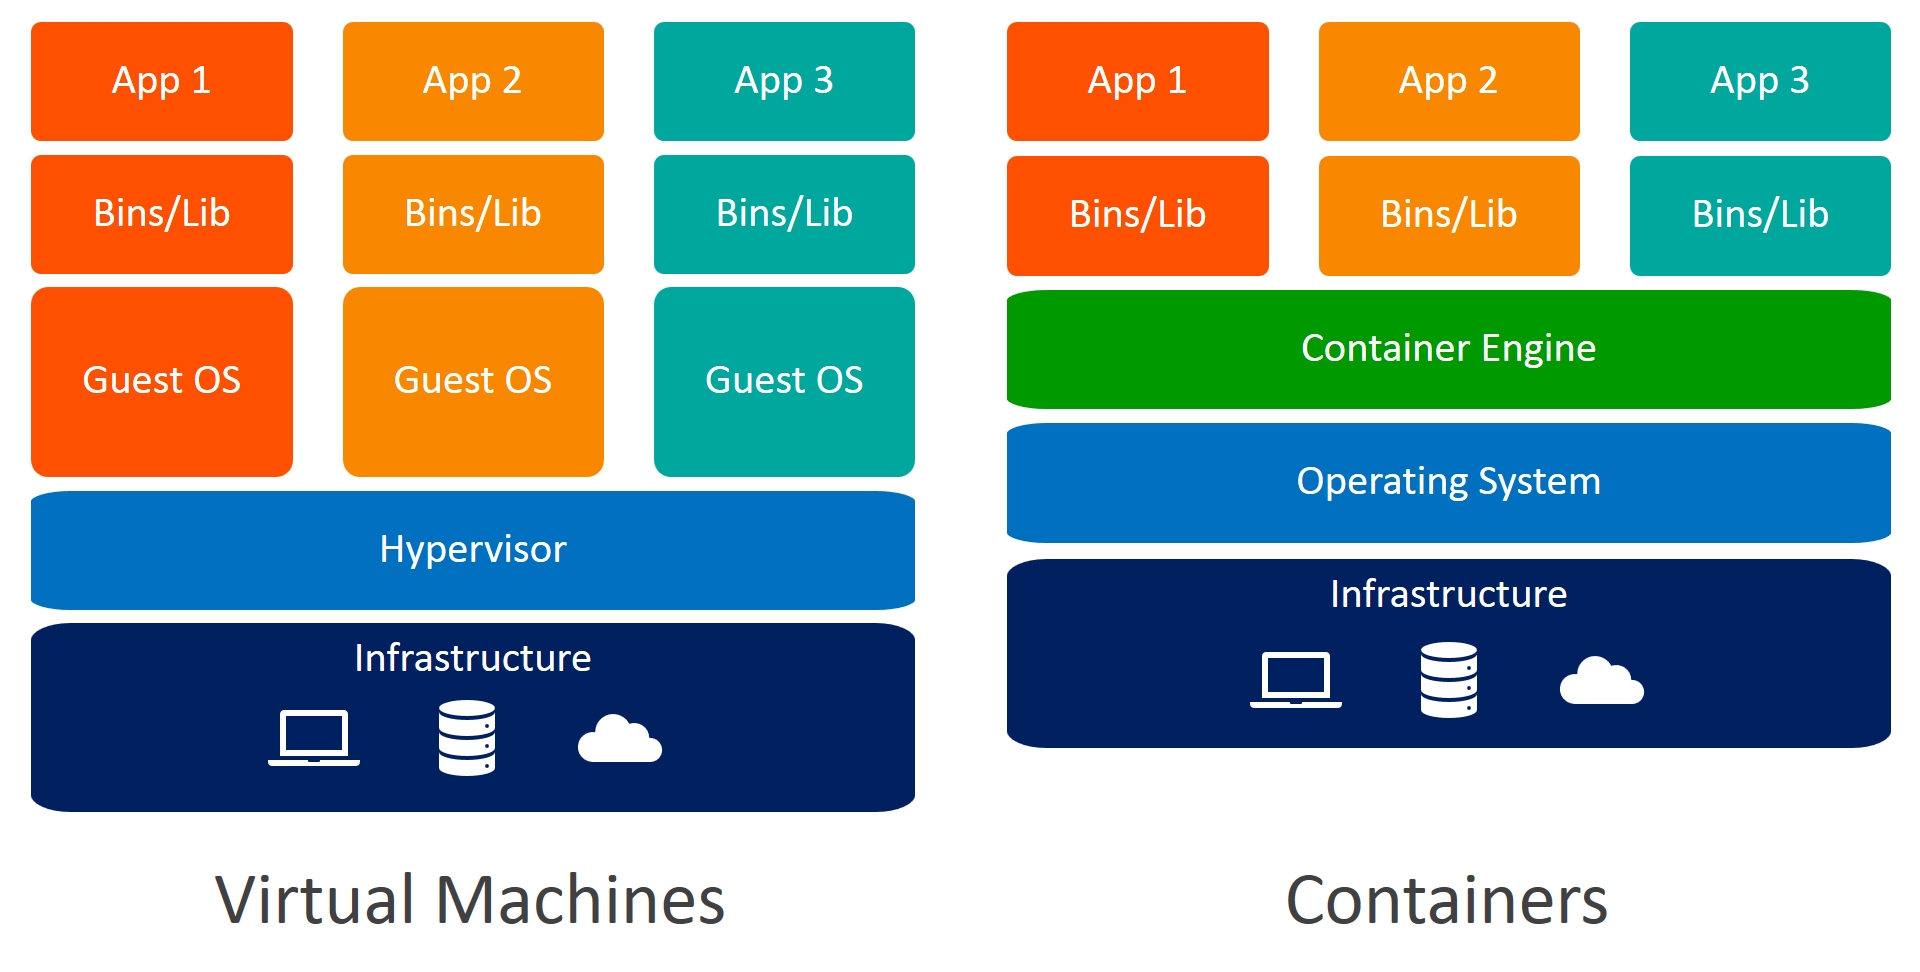
\includegraphics[width=1\textwidth]{containers-vs-virtual-machines}
	\label{fig:container-vs-vm}
\end{figure}

The starting times of virtual machines and containers are another distinction. Virtual machines typically take longer to start up because a complete operating system must be booted. In contrast, containers start up relatively instantaneously because just the containerized program needs to be started.

In conclusion, although virtual machines and containers offer virtualization and isolation, they differ in resource usage, startup time, and security, with containers providing a more portable and practical option for running applications.

\section{Source code samples}

Nulla sodales purus id mi consequat, eu venenatis odio pharetra. Cras a arcu quam. Suspendisse augue risus, pulvinar a turpis et, commodo aliquet turpis. Nulla aliquam scelerisque mi eget pharetra. Mauris sed posuere elit, ac lobortis metus. Proin lacinia sit amet diam sed auctor. Nam viverra orci id sapien sollicitudin, a aliquam lacus suscipit. Quisque ac tincidunt leo Code~\ref{src:cpp} and \ref{src:csharp}:

\lstset{caption={Hello World in C++}, label=src:cpp}
\begin{lstlisting}[language={C++}]
#include <stdio>

int main() 
{
	int c;
	std::cout << "Hello World!" << std::endl;

	std::cout << "Press any key to exit." << std::endl;
	std::cin >> c;
	
	return 0;
}
\end{lstlisting}

\lstset{caption={Hello World in C\#}, label=src:csharp}
\begin{lstlisting}[language={[Sharp]C}]
using System;
namespace HelloWorld
{
	class Hello 
	{
		static void Main() 
		{
			Console.WriteLine("Hello World!");
			
			Console.WriteLine("Press any key to exit.");
			Console.ReadKey();
		}
	}
}
\end{lstlisting}

\subsection{Algorithms}

A general Interval Branch and Bound algorithm is shown in Algorithm~\ref{alg:ibb}. An appropriate selection rule is applied in Step~\ref{step:selrule}.\\
Source of example: \href{https://www.inf.u-szeged.hu/actacybernetica/}{Acta Cybernetica (this is a hyperlink)}.

\begin{algorithm}[H]
\caption{A general interval B\&B algorithm} 
\label{alg:ibb} 
\textbf{\underline{Funct}} IBB($S,f$)
\begin{algorithmic}[1] % display line numbers before every n line, here n = 1
\State Set the working list ${\cal L}_W$ := $\{S\}$ and the final list ${\cal L}_Q$ := $\{\}$     
\While{( ${\cal L}_W \neq \emptyset$ )} \label{alg:igoend}
	\State  Select an interval $X$ from ${\cal L}_W$ \label{step:selrule}\Comment{Selection rule}  
	\State Compute $lbf(X)$ \Comment{Bounding rule}		  
	\If{$X$ cannot be eliminated} \Comment{Elimination rule}
		\State Divide $X$ into $X^j,\ j=1,\dots, p$, subintervals   \Comment{Division rule}
		\For{$j=1,\ldots,p$}
			\If{$X^j$ satisfies the termination criterion} \Comment{Termination rule}
				\State Store $X^j$ in ${\cal L}_W$ 
			\Else
				\State Store $X^j$ in ${\cal L}_W$ 
			\EndIf
		\EndFor  
	\EndIf
\EndWhile
\State \textbf{return} ${\cal L}_Q$
\end{algorithmic}
\end{algorithm}

\cleardoublepage

\chapter{Conclusion}
\label{ch:sum}

The SeleniumTest Operator is a tool that speeds the testing of web applications. This operator offers a robust and adaptable framework for developing, executing, and monitoring Selenium tests by utilizing the features of Selenium WebDriver, Kubernetes, and Prometheus.

The operator enables developers to quickly design and launch Selenium tests with multiple settings and retrieve comprehensive results, all within a Kubernetes cluster, using custom resources like SeleniumTest and SeleniumTestResult. Integrating with Prometheus makes effective monitoring and alerting based on personalized metrics and thresholds possible.

The Kubernetes API and the usage of containers further assure the portability, scalability, and simplicity of deployment of the SeleniumTest Operator in various scenarios.

Overall, the SeleniumTest Operator represents a considerable improvement in web application testing by giving developers and operators a complete and adaptable solution.
\cleardoublepage

% Acknowledgements (optional) - in case your thesis received funding or would like to express special thanks to someone
\chapter*{\acklabel}
\addcontentsline{toc}{chapter}{\acklabel}
In case your thesis received financial support from a project or the university, it is usually required to indicate the proper attribution in the thesis itself. Special thanks can also be expressed towards teachers, fellow students and colleagues who helped you in the process of creating your thesis.

% Appendices (optional) - useful for detailed information in long tables, many and/or large figures, etc.
\appendix
\chapter{Szimulációs eredmények}
\label{appx:simulation}

Lorem ipsum dolor sit amet, consectetur adipiscing elit. Pellentesque facilisis in nibh auctor molestie. Donec porta tortor mauris. Cras in lacus in purus ultricies blandit. Proin dolor erat, pulvinar posuere orci ac, eleifend ultrices libero. Donec elementum et elit a ullamcorper. Nunc tincidunt, lorem et consectetur tincidunt, ante sapien scelerisque neque, eu bibendum felis augue non est. Maecenas nibh arcu, ultrices et libero id, egestas tempus mauris. Etiam iaculis dui nec augue venenatis, fermentum posuere justo congue. Nullam sit amet porttitor sem, at porttitor augue. Proin bibendum justo at ornare efficitur. Donec tempor turpis ligula, vitae viverra felis finibus eu. Curabitur sed libero ac urna condimentum gravida. Donec tincidunt neque sit amet neque luctus auctor vel eget tortor. Integer dignissim, urna ut lobortis volutpat, justo nunc convallis diam, sit amet vulputate erat eros eu velit. Mauris porttitor dictum ante, commodo facilisis ex suscipit sed.

Sed egestas dapibus nisl, vitae fringilla justo. Donec eget condimentum lectus, molestie mattis nunc. Nulla ac faucibus dui. Nullam a congue erat. Ut accumsan sed sapien quis porttitor. Ut pellentesque, est ac posuere pulvinar, tortor mauris fermentum nulla, sit amet fringilla sapien sapien quis velit. Integer accumsan placerat lorem, eu aliquam urna consectetur eget. In ligula orci, dignissim sed consequat ac, porta at metus. Phasellus ipsum tellus, molestie ut lacus tempus, rutrum convallis elit. Suspendisse arcu orci, luctus vitae ultricies quis, bibendum sed elit. Vivamus at sem maximus leo placerat gravida semper vel mi. Etiam hendrerit sed massa ut lacinia. Morbi varius libero odio, sit amet auctor nunc interdum sit amet.

Aenean non mauris accumsan, rutrum nisi non, porttitor enim. Maecenas vel tortor ex. Proin vulputate tellus luctus egestas fermentum. In nec lobortis risus, sit amet tincidunt purus. Nam id turpis venenatis, vehicula nisl sed, ultricies nibh. Suspendisse in libero nec nisi tempor vestibulum. Integer eu dui congue enim venenatis lobortis. Donec sed elementum nunc. Nulla facilisi. Maecenas cursus id lorem et finibus. Sed fermentum molestie erat, nec tempor lorem facilisis cursus. In vel nulla id orci fringilla facilisis. Cras non bibendum odio, ac vestibulum ex. Donec turpis urna, tincidunt ut mi eu, finibus facilisis lorem. Praesent posuere nisl nec dui accumsan, sed interdum odio malesuada.
\cleardoublepage

% Bibliography (mandatory)
\phantomsection
\addcontentsline{toc}{chapter}{\biblabel}
\printbibliography[title=\biblabel]
\cleardoublepage

% List of figures (optional) - useful over 3-5 figures
\phantomsection
\addcontentsline{toc}{chapter}{\lstfigurelabel}
\listoffigures
\cleardoublepage

% List of tables (optional) - useful over 3-5 tables
\phantomsection
\addcontentsline{toc}{chapter}{\lsttablelabel}
\listoftables
\cleardoublepage

% List of algorithms (optional) - useful over 3-5 algorithms
\phantomsection
\addcontentsline{toc}{chapter}{\lstalgorithmlabel}
\listofalgorithms
\cleardoublepage

% List of codes (optional) - useful over 3-5 code samples
\phantomsection
\addcontentsline{toc}{chapter}{\lstcodelabel}
\lstlistoflistings
\cleardoublepage

% List of symbols (optional)
%\printnomenclature

\end{document}
